\documentclass[11pt]{article}
\usepackage{url,amsmath,amsfonts,amsthm,graphicx}
\usepackage[a4paper,margin=1in]{geometry}

\newcommand{\ulp}{{\upshape(}}
\newcommand{\urp}{\/{\upshape)}}
\newtheorem{thm}{Theorem}
\newtheorem{prop}{Proposition}
\newtheorem{lem}{Lemma}
\newtheorem{conj}{Conjecture}
\theoremstyle{definition}
\newtheorem{defn}{Definition}
\newtheorem*{note}{Note}
\newtheorem*{notes}{Notes}
\newtheorem{exa}{Example}
\newtheorem{exas}[exa]{Examples}
\DeclareMathOperator*{\Sp}{\mathrm{Sp}}
\DeclareMathOperator*{\NP}{\mathrm{NP}}
\DeclareMathOperator*{\lch}{\mathrm{lch}}
\DeclareMathOperator*{\val}{\mathrm{val}}
\DeclareMathOperator*{\Tr}{\mathrm{Tr}}
\author{Jonathan Nimmo}
\title{Periodic discrete KdV equation}
\date{}
\begin{document}
\maketitle
\tableofcontents
\section{Peroidic discrete Schr\"odinger equation}

Consider the inhomogeneous second order difference equation (discrete Schr\"odinger equation)
\begin{equation}\label{eq: 2nd diff}
\phi_{j-1}-2\phi_{j}+(1+\lambda)\phi_{j+1}=a_{j}\phi_{j},
\end{equation}
where $i\in\mathbb Z$. The homogeneous version of \eqref{eq: 2nd diff}, 
\begin{equation}\label{eq: 2nd diff hom}
\phi_{j-1}-2\phi_{j}+(1+\lambda)\phi_{j+1}=0,
\end{equation}
has solutions $\phi_{j}=(1\pm i \sqrt\lambda)^{-j}$ and in particular, mimicking trigonometric functions $\cos$ and $\sin$, we define
\begin{align}
	\cos_\lambda(j)&=\frac12((1-i\sqrt\lambda)^{-j}+(1+i\sqrt\lambda)^{-j})\\
	\sin_\lambda(j)&=\frac1{2i}((1-i\sqrt\lambda)^{-j}-(1+i\sqrt\lambda)^{-j}).
\end{align}
It is straightforward to verify the properties
\begin{gather}
\label{eq:trig prop1}
	\cos_\lambda(0)=1,\quad \sin_\lambda(0)=0,\quad\cos_\lambda(-1)=1,\quad \sin_\lambda(-1)=-\sqrt\lambda,\\
\label{eq:trig prop2}
	\cos_\lambda(j)-\cos_\lambda(j-1)=-\sqrt\lambda\sin_\lambda(j),\quad\sin_\lambda(j)-\sin_\lambda(j-1)=\sqrt\lambda\cos_\lambda(j),
\end{gather}
and hence $\cos_\lambda(j-j_0)$ and $\sin_\lambda(j-j_0)/\sqrt\lambda$ are the solutions of \eqref{eq: 2nd diff hom} satisfying the boundary conditions
\begin{equation}
	\phi_{j_0}=1,\quad \Delta\phi_{j_0}=0,\qquad
	\phi_{j_0}=0,\quad \Delta\phi_{j_0}=1,
\end{equation}
respectively, in which $\Delta$ denotes the backwards difference operator $\Delta f_{j}:=f_{j}-f_{j-1}$.

\subsection{Green's function and the fundamental matrix}
Next we solve the inhomogeneous version by means of a Green's function. We seek a solution of
\begin{equation}\label{eq: 2nd diff delta}
\phi_{j-1}-2\phi_{j}+(1+\lambda)\phi_{j+1}=\delta_{j,j_0},
\end{equation}
in the form
\begin{equation}
\phi_{j}=
\begin{cases}
0                         & j<j_0\\
\alpha(1-i\sqrt\lambda)^{-j}+\beta(1+i\sqrt\lambda)^{-j} & j>j_0	
\end{cases}
\end{equation}
``Continuity'' at $j=j_0$ dictates that 
\begin{equation}
\alpha(1-i\sqrt\lambda)^{-j_0}+\beta(1+i\sqrt\lambda)^{-j_0}=0,
\end{equation}
and so
\begin{equation}
\phi_{j}=
\begin{cases}
0                         & j\le j_0\\
\gamma\sin_\lambda(j-j_0)            & j>j_0.	
\end{cases}
\end{equation}
Taking the sum of \eqref{eq: 2nd diff delta} over any interval $\{m,\dots,n\}\subset\mathbb Z$ containing $j_0$ gives
\begin{equation}
\Delta\phi_{n+1}-\Delta\phi_{m}+\lambda\sum_{j=m}^{n}\phi_{j+1}=1,	
\end{equation}
and so taking $m=n=j_0$ gives
\begin{equation}
\bigl((1+\lambda)\phi(j_0+1)=)\gamma(1+\lambda)\sin_\lambda(1)=1.
\end{equation}
Hence we obtain the Green's function 
\begin{equation}
G(j;j_0,\lambda)=
\begin{cases}
0                         & j\le j_0\\
\dfrac{\sin_\lambda(j-j_0)}{\sqrt\lambda} & j>j_0	
\end{cases}
\end{equation}
\begin{prop}
The solutions satisfying the inhomogeneous equation \eqref{eq: 2nd diff} and boundary conditions $c_{j_0}=1$, $\Delta c_{j_0}=0$ and $s_{j_0}=0$, $\Delta s_{j_0}=1$, are
\begin{equation}\label{eq: c_{j}}
c_{j}=\cos_\lambda(j-j_0)+
\begin{cases}
\displaystyle
\sum_{m=j_0}^{j-1}\frac{\sin_\lambda(j-m)}{\sqrt\lambda} a_{m} c_{m}  &  j\ge j_0\\
\displaystyle
-\sum_{m=j+1}^{j_0-1}\frac{\sin_\lambda(j-m)}{\sqrt\lambda} a_{m} c_{m}  &  j< j_0	
\end{cases}
\end{equation}
and
\begin{equation}\label{eq: s_{j}}
s_{j}=\frac{\sin_\lambda(j-j_0)}{\sqrt\lambda}+
\begin{cases}
\displaystyle
\sum_{m=j_0+1}^{j-1}\frac{\sin_\lambda(j-m)}{\sqrt\lambda} a_{m} s_{m}  &  j\ge j_0\\
\displaystyle
-\sum_{m=j+1}^{j_0-1}\frac{\sin_\lambda(j-m)}{\sqrt\lambda} a_{m} s_{m}  &  j< j_0	
\end{cases}
\end{equation}
respectively.
\end{prop}
\begin{proof}
Straightforward direct calculations. For example, $c_{j}$ for $j+1<j_0$: using properties \eqref{eq:trig prop1}--\eqref{eq:trig prop2}, the boundary conditions are satisfied and $c_{j+1}-2c_{j}+c_{j-1}$ gives
\begin{align*}
&\cos_\lambda(j+1-j_0)-2\cos_\lambda(j-j_0)+\cos_\lambda(j-1-j_0)\\
&\qquad-\left(\sum_{m=j+2}^{j_0-1}\frac{\sin_\lambda(j+1-m)}{\sqrt\lambda}-2\sum_{m=j+1}^{j_0-1}\frac{\sin_\lambda(j-m)}{\sqrt\lambda}+\sum_{m=j}^{j_0-1}\frac{\sin_\lambda(j-1-m)}{\sqrt\lambda}\right) a_{m} c_{m}\\	
&=-\lambda\cos_\lambda(j+1-j_0)-\sum_{m=j+2}^{j_0-1}\left(\frac{\sin_\lambda(j+1-m)}{\sqrt\lambda}-2\frac{\sin_\lambda(j-m)}{\sqrt\lambda}+\frac{\sin_\lambda(j-1-m)}{\sqrt\lambda}\right) a_{m} c_{m}\\
&\qquad+2\frac{\sin_\lambda(-1)}{\sqrt\lambda}a_{j+1}c_{j+1}-\frac{\sin_\lambda(-1)}{\sqrt\lambda}a_{j}c_{j}
-\frac{\sin_\lambda(-2)}{\sqrt\lambda}a_{j+1}c_{j+1}\\
&=-\lambda\cos_\lambda(j+1-j_0)+\lambda\sum_{m=j+2}^{j_0-1}\frac{\sin_\lambda(j+1-m)}{\sqrt\lambda}
+a_{j}c_{j}\\
&=-\lambda c_{j+1}+a_{j}c_{j},
\end{align*}
as required.
\end{proof}
\begin{note}
The expressions \eqref{eq: c_{j}} and \eqref{eq: s_{j}} are recurrence relations which may be used to determine \emph{explicit} expressions for $c_{j}$ and $s_{j}$ for any $j\in\mathbb Z$.
\end{note}
\begin{exa}
We have 
\begin{align}
	c_{j_0+1}&=\cos_\lambda(1)+\frac{\sin_\lambda(1)}{\sqrt\lambda}a_{j_0}c_{j_0}\\
	&=\frac{1+a_{j_0}}{1+\lambda},\\
\intertext{and}
	c_{j_0+2}&=\cos_\lambda(2)+\frac{\sin_\lambda(2)}{\sqrt\lambda}a_{j_0}c_{j_0}
	+\frac{\sin_\lambda(1)}{\sqrt\lambda}A(j_0+1)c(j_0+1)\\
	&=\frac{1-\lambda+2a_{j_0}+A(j_0+1)+a_{j_0}A(j_0+1)}{(1+\lambda)^2}.
\end{align}
Similarly, $c(j_0-1)=1/(1+\lambda)$ and $s(j_0+2)=(2+a_{j_0})/(1+\lambda)^2$.
\end{exa}
\begin{defn}
The fundamental matrix for \eqref{eq: 2nd diff} is
\begin{equation}
	\Phi_{j}:=
	\begin{pmatrix}
	c_{j}&s_{j}\\
	\Delta c_{j}&\Delta s_{j},
	\end{pmatrix}
\end{equation}
and is such that $\Phi_{j_0}=I$.
\end{defn}

\subsection{Casoratian relation}
For any two solutions $\phi_{j}$, $\psi_{j}$ of \eqref{eq: 2nd diff} we can define a solution matrix whose determinant is the Casoratian
\begin{equation}
C(\phi_{m},\psi_{m})=\det
\begin{pmatrix}
\phi_{m}&\psi_{m}\\
\Delta\phi_{m}&\Delta\psi_{m}
\end{pmatrix}	
=\phi_{m-1}\psi_{m}-\phi_{m}\psi_{m-1}.
\end{equation}
Also we have
\begin{align}
\psi_{j}&(\phi_{j-1}-2\phi_{j}+(1+\lambda)\phi_{j+1})\\
-\phi_{j}&(\psi_{j-1}-2\psi_{j}+(1+\lambda)\psi_{j+1})=0,
\end{align}
which may be written as
\begin{equation}\label{eq: cas}
C(\phi_{j},\psi_{j})=(1+\lambda)C(\phi_{j+1},\psi_{j+1}),
\end{equation}
where  
\begin{equation}
C(\phi_{j},\psi_{j}):=\phi_{j-1}\psi_{j}-\phi_{j}\psi_{j-1},
\end{equation}
is the Casoratian of the solutions.


\subsection{Periodic boundary conditions and the monodromy matrix}
Now suppose that the potential $a_{j}$ is periodic of period $N$ so that for all $j$, $a_{j+N}=a_{j}$. Although the system is periodic, its solutions are not. However we have that $\Phi_{j+N}$ must also be a solution matrix and hence can be expressed in terms of the fundamental matrix $\Phi_{j}$ as follows:
\begin{equation}
\Phi_{j+N}=\Phi_{j}M,
\end{equation}
where $M$ is a constant matrix. Since $\Phi_{j_0}=I$, it follows that
\begin{equation}
M=\Phi(j_0+N),
\end{equation}
and $M$ is called the \emph{monodromy matrix}.

\begin{prop}
The fundamental matrix $\Phi_{j}$ has determinant $(1+\lambda)^{j_0-j}$. In particular, the determinant of the monodromy matrix is
\begin{equation}
	\det M=(1+\lambda)^{-N}.
\end{equation}
\end{prop}
\begin{proof}
From \eqref{eq: cas} with $\phi_{j},\psi_{j}$ taken to be $c_{j},s_{j}$,
\begin{equation}
\det\Phi_{j}=(1+\lambda)\det\Phi_{j+1},
\end{equation}
and by definition $\Phi_{j_0}=I$. The result follows by induction. 
\end{proof}

\subsection{Floquet multipliers and the spectral equation}
Let $\mu$ be an eigenvalue (Floquet multiplier) of the monodromy matrix $M$. Then there exists a non-trivial eigensolution 
$\psi_j$ such that for all $j$, $\psi_{N+j} = \mu\psi_j$ and more generally,
\begin{equation}
\psi_{j+kN} = \mu^k\psi_j,	
\end{equation}
for any integer $k$. The eigenfunction $\psi_j$ is bounded for all $j$ if and only if $|\mu|=1$, and it is called a 
\emph{Bloch function}. The eigenvalues $\mu$ are the roots of the spectral equation
\begin{equation}
	\det(M - \lambda I) = \lambda^2 - \Tr(M)\lambda + \det(M) = 0.
\end{equation}
We already calculated that $\det(M)=(1+\lambda)^{-N}$ and it is therefore important to study the properties of $\Tr(M) = c_{j_0+N}+ \Delta s_{j_0+N}$. (To do: Show that $\Tr(M)$ is also independent of $j_0$)

\section{Binary bracelets}
Consider the set of all words $W_n$ of length $n$ in an alphabet with two symbols, $1$ and $0$, say. These words are acted on by permutations which reorder the $n$ symbols. The orbits of words under the action of the dihedral group $D_n$ split $W_n$ into equivalence classes and the lexicographically lowest member is called a (binary) \emph{bracelets} \cite{}.  For example, $b=01011$ is the bracelet representing the equivalence class
\begin{equation}\label{eq:Cb}
C_b=\{11010,01101,10110,01011,10101\}.	
\end{equation}
Let $\mathbf B_2(n)$ denote the set of all binary bracelets of length $n$ and let $\mathbf B^\times_2 (n)$ denote the subset which excludes the null bracelet $00 \dots 0$. This subset will be used later.

It is known \cite{} that the number of binary bracelets are given by the formula
\begin{equation}
	B_2(n)=|\mathbf B_2(n)|=\frac1{2n}\sum_{d\vert n}\varphi(d)2^{n/d}+  
	\begin{cases}
		3\;2^{n/2-2}&n\text{ even}\\
		2^{_{n-1}/2}&n\text{ odd},
	\end{cases}
\end{equation}
where $\varphi$ is Euler's totient function. For example,
\begin{center}
\begin{tabular}{c|ccccccccccccccccc}
$n$&1&2&3&4&5&6&7&8&9&10&11&12&13&14&15\\
\hline
$B_2(n)$&2&3&4&6&8&13&18&30&46&78&126&224&380&687&1224
\end{tabular}	
\end{center}
All of the binary bracelets of length 7 are illustrated in Figure~\ref{fig:b7}.
\begin{figure}[htbp]
\centering
		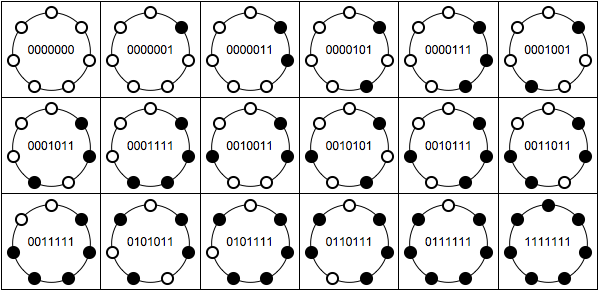
\includegraphics[width=6in]{B7.png}
		\caption{All of the binary bracelets of length 7.\label{fig:b7}}
\end{figure}

To each member of the equivalence class of a bracelet $b\in\mathbf B_2(n)$ associate a monomial in variables $a_0,a_1\dots,a_{n-1}$. For a $1$ in position $0\le k\le n-1$, $a_k$ is included in the monomial and otherwise $a_k$ is omitted. The monomials are summed over the equivalence to class to obtain a unit coefficient polynomial $p(b)$. For example, with $b=01011$ as given above, with equivalence class (or orbit) $C_b$ given by \eqref{eq:Cb}, we have
\begin{equation}
 	p(b)=a_0a_1a_3+a_1a_2a_4+a_0a_2a_3+a_1a_3a_4+a_0a_2a_4.
 \end{equation} 
By construction, these polynomials $p(b)$ are dihedral invariants in the same way that elementary symmetric polynomials are invariants of the full symmetric group.
\begin{notes}		
1. Although there is only one elementary symmetric function (Sn invariant) of degree $0 \le k \le n$, there may be several
$D_n$ invariants of the same degree.

2. The invariants of dihedral group $D_n$ are precisely elementary symmetric functions for $n \le 3$ and so the first case in which the restricted symmetric is apparent is at $n = 4$. For example, $p(0101) = a_0a_2 + a_1a_3$ is the simplest dihedral inveriant that is not an elementary symmetric function.	
\end{notes}		
There are two partitions associated with each bracelet $b \in B_2(n)$; $\alpha(b)$ records the lengths of the blocks of 
consecutive 1s and $\beta(b)$ the lengths of the blocks of 0s. For example, if $b = 0001100101$, then $\alpha(b) = (212)$ 
and $\beta(b) = (321)$. However, this pair of partitions does not uniquely characterise the bracelet since, for example, $0001101001$ has the same associated partitions as the previous example.

For non-negative integers $j$, define
\begin{equation}
f_\lambda(j)=-\frac{\sin_\lambda(-j-1)}{\sqrt\lambda}=\sum_{k=0}^{[j/2]}(-1)^k\binom{j+1}{2k+1}\lambda^k.
\end{equation}
which is clearly an integer-coefficient polynomial in $\lambda$. The first few such polynomials are
\begin{center}
\begin{tabular}{c|ccccccc}
$j$&0&1&2&3&4&5&6\\\hline
$f_\lambda(j)$& $1$&$2$&$3-\lambda$&$4-4\lambda$&$5-10\lambda+\lambda^2$&$6-20\lambda+6\lambda^2$&$7-35\lambda+21\lambda^2-\lambda^3$	
\end{tabular}
\end{center}
We also extend this definition to partitions $\beta = (\beta_1, \dots, \beta_p)$ and thereby to bracelets $b$ in a natural way:
\begin{equation}
f_\lambda(\beta) := 􏰅\prod_{k=1}^p f_\lambda(\beta_k),\qquad f_\lambda(b):=f_\lambda(\beta(b)).
\end{equation}

\begin{conj}
The trace of the monodromy matrix is given by
\begin{equation}
	\Tr \Phi(N)=2\cos_\lambda(N)+\frac1{(1+\lambda)^N}\sum_{b\in\mathbf B^\times_2(N)} f_\lambda(b) p(b).
\end{equation}
\end{conj}
This conjecture has been verified by computer for $N \le 20$. In the case $N=20$, the sum is over $27,011$ bracelets.
\begin{note}		
The trace of $M$ in the case of trivial potential $a_j=0$ is given by the term $2\cos_\lambda(N)=\cos_\lambda(N)+\Delta\sin_\lambda(N)/ \sqrt\lambda$.	
\end{note}		

The formula can be written in a slightly more compact way as 
\begin{equation}
	\Tr \Phi(N)=\frac{2\cos_\lambda(-N)+\sum_{b\in\mathbf B^\times_2(N)} f_\lambda(b) p(b)}{(1+\lambda)^N}.
\end{equation}
since $(1 + \lambda)^N\cos_\lambda(N) = \cos_\lambda(-N)$. In this expression the numerator is polynomial in $\lambda$.

\begin{exa}
Take $N = 3$. We have $\mathbf B^\times_2(3) = \{001, 011, 111\}$ and so
\begin{center}
\begin{tabular}{c|ccc}
$b$&001&011&111\\\hline	
$p(b)$&$a_0 +a_1 +a_2$ &$a_0a_1 +a_0a_2 +a_1a_2$&$a_0a_1a_2$\\
$\beta(b)$&$(2)$&$(1)$&$\emptyset$\\
$f_\lambda(b)$&$3-\lambda$&$2$&$1$
\end{tabular}
\end{center}
Therefore, the conjecture is that
\begin{align*}
\Tr(M)=c_3 +\Delta s_3 &= \frac{2\cos_\lambda(−3)+f_\lambda(001)p(001)+f_\lambda(011)p(011)+f_\lambda(111)p(111)}{(1+\lambda)^3}\\
&=\frac{2-6\lambda+(3-\lambda)(a_0 +a_1 +a_2)+2(a_0a_1 +a_0a_2 +a_1a_2)+a_0a_1a_2}{(1+\lambda)^3}	
\end{align*}
This can be verified by direct calculation using the recursive definitions \eqref{eq: c_{j}} and \eqref{eq: s_{j}}.
Similarly for $N=4$, 
\begin{align*}
\Tr(M)&=\bigl(2\cos_\lambda(−4)+f_\lambda(0001)p(0001)+f_\lambda(0011)p(0011)+f_\lambda(0101)p(0101)\\
&\qquad+f_\lambda(0111)p(0111)+f_\lambda(1111)p(1111)\bigr)/(1+\lambda)^4\\
&=\bigl(2-12\lambda+2\lambda^2+(4-4\lambda)(a_0 +a_1 +a_2+a_3)+(3-\lambda)(a_0a_1 +a_1a_2 +a_2a_3+a_3a_0)\\
&\qquad+4(a_0a_2+a_1a_3)+2(a_0a_1a_2+a_1a_2a_3+a_2a_3a_0+a_3a_0a_1)+a_0a_1a_2a_3\bigr)/(1+\lambda)^4.	
\end{align*}

\end{exa}
\end{document}